\documentclass{beamer}
\usetheme[hideothersubsections]{PaloAlto}
\usecolortheme{albatross}

\usepackage{etoolbox}

\definecolor{Antra}{RGB}{105,105,105}
\definecolor{AntraB}{RGB}{105,105,125}
\definecolor{Gris}{RGB}{80,80,85}

\setbeamercolor*{structure}{fg=Antra!50,bg=AntraB}
\setbeamercolor*{palette primary}{use=structure,fg=white,bg=Gris}
\setbeamercolor*{background canvas}{bg=Antra,fg=Antra}
\setbeamercolor*{normal text}{bg=AntraB,fg=Antra!10}
\setbeamercolor*{navigation symbols}{bg=AntraB,fg=Antra!10}

\beamertemplatenavigationsymbolsempty


\title[Final Presentation]{HOVERCRAFT PROJECT\\Final Presentation}
\author[]{Florian POUTHIER - Tristan DRUSSEL\\ \tiny florian.pouthier@insa-strasbourg.fr - tristan.drussel@insa-strasbourg.fr}
\date{Mai, 27th, 2020}
\institute{4th Year Electrical Engeenering \\ INSA Strasbourg}

\setbeamertemplate{footline}
{
	\leavevmode% 
	\begin{beamercolorbox}[wd=0.3333\paperwidth,left,ht=0.025\paperheight,dp=0.0125\paperheight]{palette primary}
	   	\hspace*{2em}\insertauthor
	\end{beamercolorbox}
	\begin{beamercolorbox}[wd=0.3333\paperwidth,center,ht=0.025\paperheight,dp=0.0125\paperheight]{AntraB}
		\hspace*{2em} \textbf{\insertframenumber} \hspace*{2em}
	\end{beamercolorbox}
	\begin{beamercolorbox}[wd=0.3333\paperwidth,right,ht=0.025\paperheight,dp=0.0125\paperheight]{palette primary}
		\insertshorttitle\hspace*{2em}
	\end{beamercolorbox}
	\vskip0pt
}
\setbeamertemplate{caption}[numbered]

\begin{document}
	\begin{frame}[noframenumbering,plain]
		\titlepage
	\end{frame}
	\author[]{Tristan DRUSSEL}
	\begin{frame}
		\frametitle{Overview}
	%Contexte du projet
	%organisation du travail,problématique, questionnement reformulation du rpbleme
		\begin{columns}[T]
	  		\begin{column}{0.5\textwidth}
	  		\begin{itemize}
	  			\item Hovercraft realisation
				\item Implementation of Power electronic and Digital electronic
	  		\end{itemize}
	  		\end{column}
	  		\begin{column}{0.5\textwidth}
	  			\begin{figure}
	    			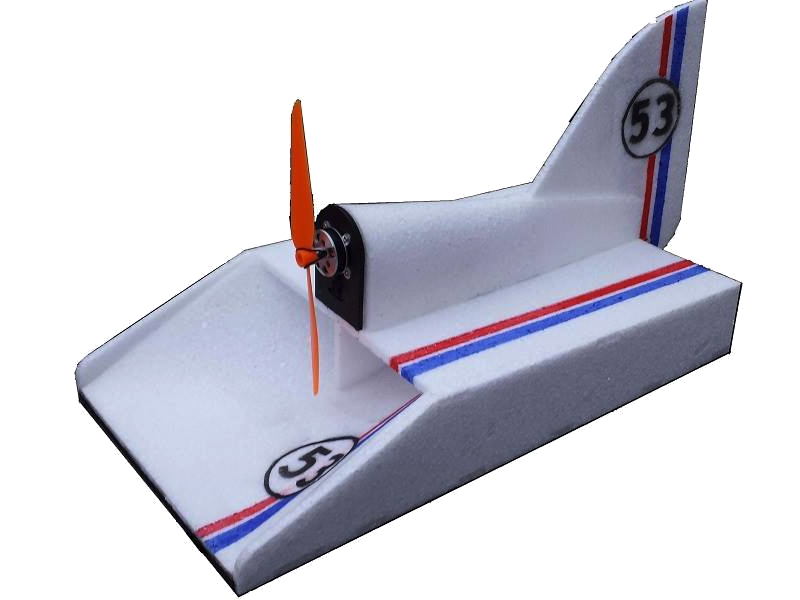
\includegraphics[width=0.8\textwidth]{../Illus/Chticat.png}
	    			\caption{Picture of a real Chticat}
	    		 \end{figure}
	  		\end{column}
		\end{columns}
	\end{frame}
	\begin{frame}{Summary}
	%Plan d'intervention succinct
		\setcounter{tocdepth}{1}
		\tableofcontents
	\end{frame}
	\begin{frame}{Mechanical aspect}
		\section[Mechanics]{Mechanical aspect}
		\subsection{CAD}
		\begin{columns}[T]
	  		\begin{column}{0.5\textwidth}
		    	\begin{itemize}
		    		\item Blueprint download
		    		\item Modification and adaptation
		    	\end{itemize}
		    	\begin{figure}
	    			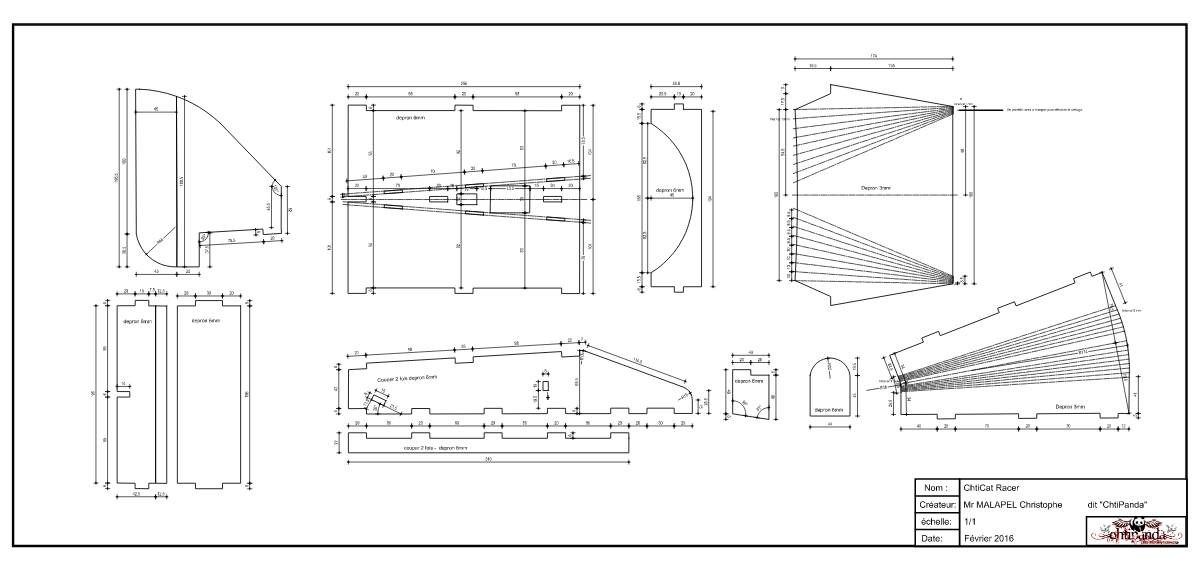
\includegraphics[width=0.8\textwidth]{../Illus/Source_Chticat.png}
	    			\caption{Blueprint of the Chticat}
	    		 \end{figure}
	  		\end{column}
	  		\begin{column}{0.5\textwidth}
	    		\begin{figure}
	    			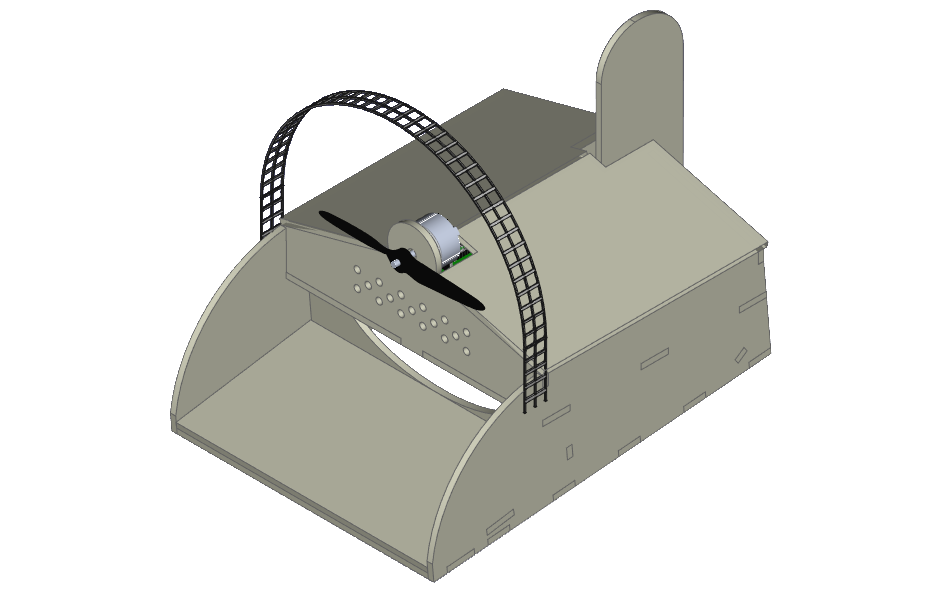
\includegraphics[width=0.8\textwidth]{../Illus/AeroProt.png}
	    			\caption{Our adapted and modified model}
	    		 \end{figure}
	  		\end{column}
		\end{columns}
		
	\end{frame}
	\begin{frame}{Digital Electronics}
		\section[Digital Elec]{Digital Electronics}
		Communication between all elements:
		\begin{itemize}
			\item smartphone app
	  		\item Bluetooth receptor: \texttt{HC-05}
			\item \texttt{PIC16F1619}
			\item \texttt{dsPIC10F2030}
	  	\end{itemize}
	  	Inverter handling
	\end{frame}
	\begin{frame}{Digital Electronics:}
		\framesubtitle{Bluetooth Communication}
		\subsection[Bluetooth]{Bluetooth Communication}
		\begin{columns}[T]
	  		\begin{column}{0.5\textwidth}
		    	\begin{itemize}
		    		\item Smartphone Controlled
		    	\end{itemize}
		    	\begin{figure}
		    		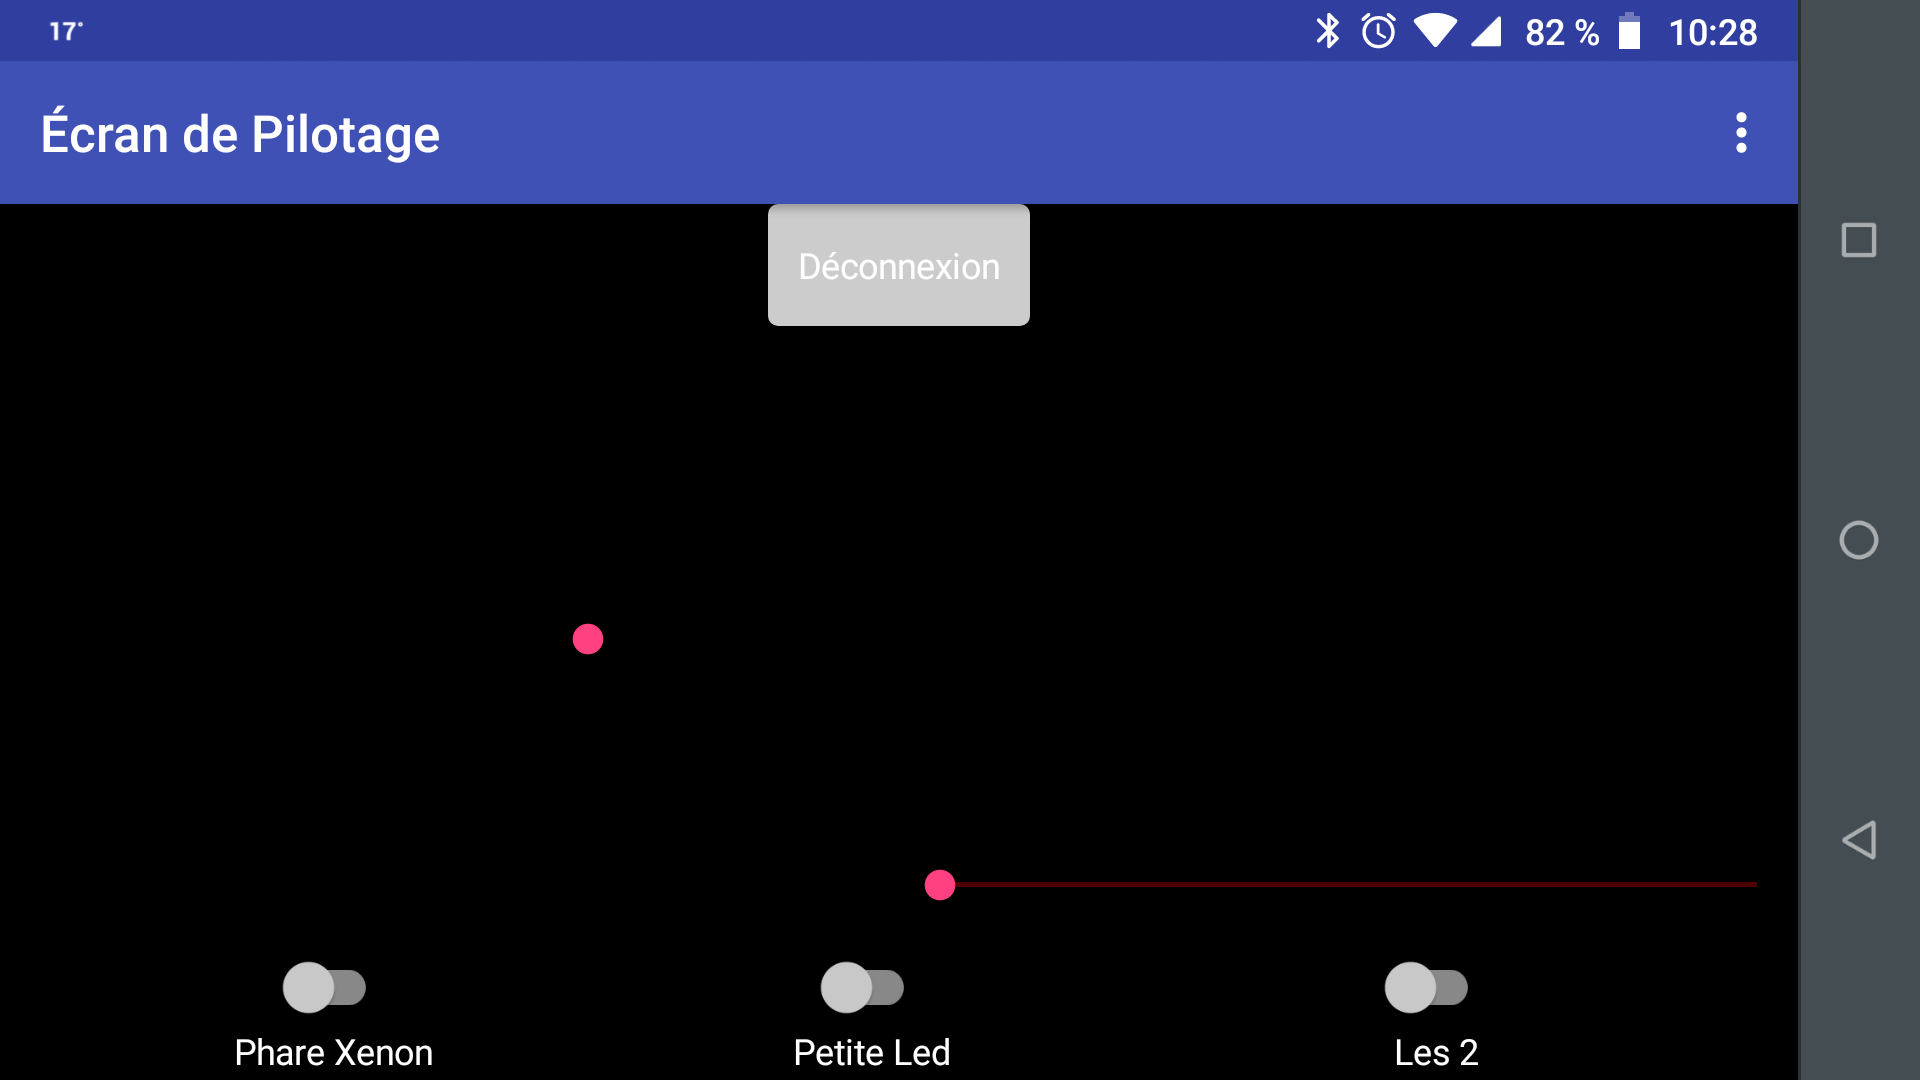
\includegraphics[width=0.8\textwidth]{../Illus/AppPilotage.png}
	    			\caption{Driving screen on the App}
	    		 \end{figure}
	  		\end{column}
	  		\begin{column}{0.5\textwidth}
	  			\begin{figure}
	    			\hspace*{2em}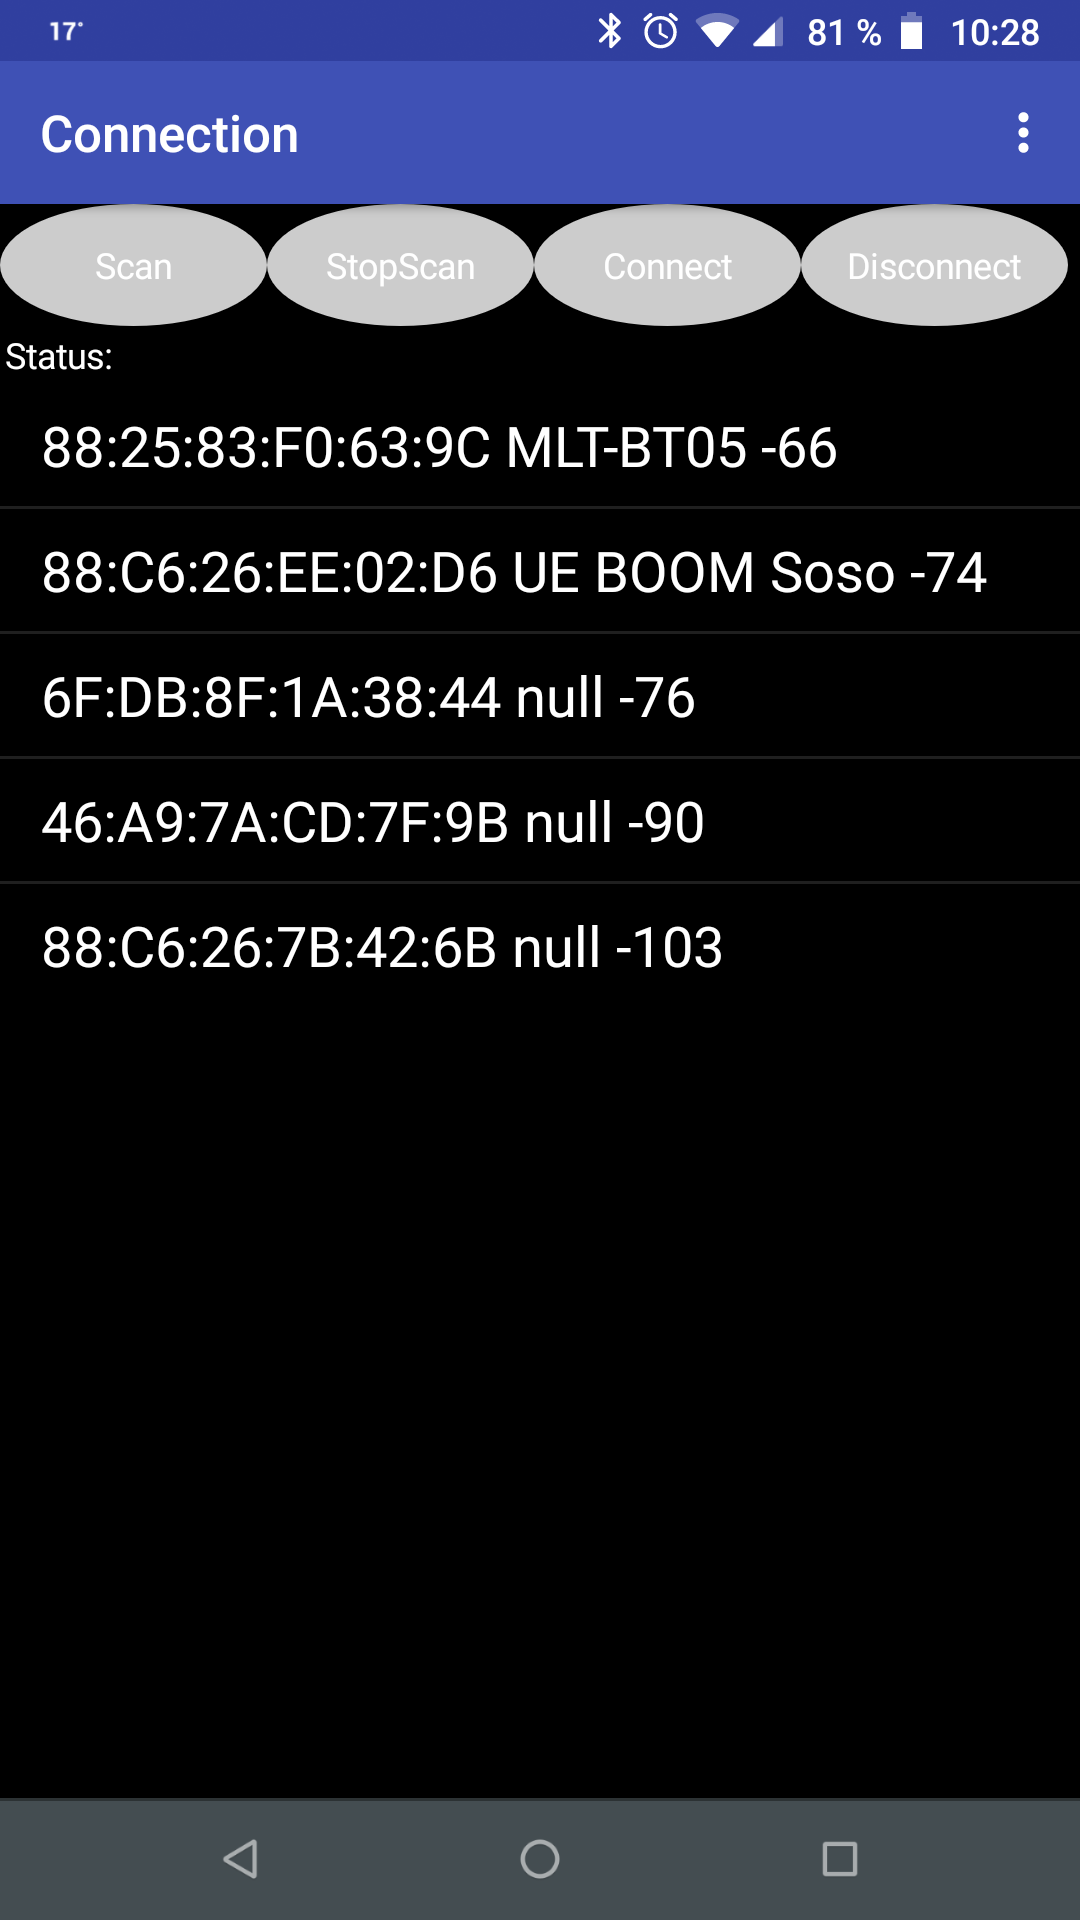
\includegraphics[height=0.8\textheight]{../Illus/AppConnection.png}
	    			\caption{Connection Screen on the application}
	    		\end{figure}
	  		\end{column}
		\end{columns}
		
	\end{frame}
	\begin{frame}{Digital Electronics:}
		\framesubtitle{Serial Communication}
		\subsection[Serial]{Serial Communication}
		\begin{itemize}
		    \item Communication between Bluetooth receptor and \texttt{PIC16F1619}
		\end{itemize}
		\begin{columns}[T]
	  		\begin{column}{0.5\textwidth}
		    	\begin{figure}
		    		
\includegraphics[width=0.45\textwidth]{../Illus/BluetoothLogo.png}
	    			\caption{Bluetooth Logo}
	    		 \end{figure}
	  		\end{column}
	  		\begin{column}{0.5\textwidth}
	  			\begin{figure}
	    			\hspace*{2em}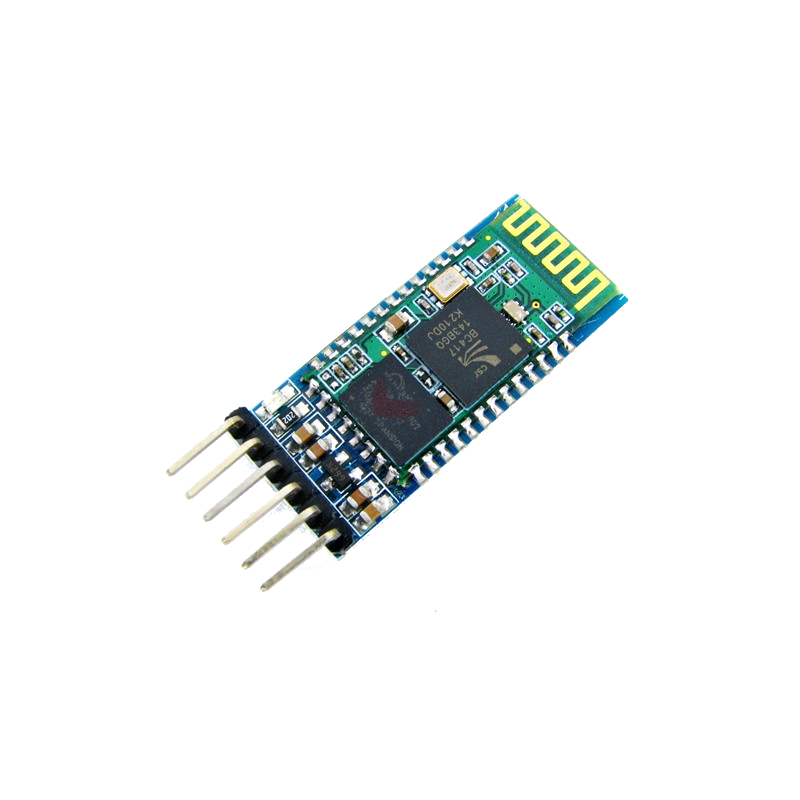
\includegraphics[width=0.7\textwidth]{../Illus/HC05.png}
	    			\caption{Bluetooth receptor \texttt{HC-05}}
	    		\end{figure}
	  		\end{column}
	  	\end{columns}
	\end{frame}
	\begin{frame}{Digital Electronics:}
	\framesubtitle{\textit{Serial Peripheral Interface} Communication}
		\subsection[SPI]{Communication SPI}
		\begin{itemize}
		    \item Communication between \texttt{PIC16F1619} and \texttt{dsPIC10F2030}
		    \setlength{\unitlength}{0.75mm}
		    \begin{figure}
		    
		\begin{center}
			\begin{picture}(125,35)
			\tiny
			\multiput(0,10)(75,0){2}{
				\multiput(5,0)(5,0){8}{\framebox(5,5){}}
				\put(23,-2){\vector(1,0){8}}
			}
			
			\put(42.5,10){\line(0,-1){5}}
			\put(82.5,5){\vector(0,1){5}}
			\put(42.5,5){\line(1,0){40}}
			
			\put(7.5,20){\vector(0,-1){5}}
			\put(117.5,15){\line(0,1){5}}
			\put(7.5,20){\line(1,0){110}}
			
			\multiput(55,30)(1.5,2){2}{
				\multiput(0,0)(3,0){5}{
					\put(0,0){\line(1,0){1.5}}				
				}			
			}
			\put(49,27.5){\vector(1,0){29}}
			
			\multiput(55,30)(1.5,0){10}{
					\put(0,0){\line(0,1){2}}				
				}
			\multiput(0,0)(75,0){2}{
				\multiput(3.5,0)(45.5,0){2}{
					\multiput(0,0)(0,3){12}{\line(0,1){1.75}}			
				}
				\multiput(3.5,0)(0,35){2}{
					\multiput(0,0)(3,0){15}{\line(1,0){1.75}}			
				}
			}
			
			\put(20,32){\texttt{PIC16F1619}}
			\put(100,32){\texttt{dsPIC10F2030}}
			\put(59,24.5){SCK}
			\put(59,17){MISO}
			\put(59,2.5){MOSI}
			\end{picture}
		\end{center}
		\caption{SPI}
	\end{figure}
		\end{itemize}
	\end{frame}
	\begin{frame}{Digital Electronics:}
		\framesubtitle{Inverter handling}
		\subsection[Inverter]{Inverter handling}
		\begin{columns}[T]
	  		\begin{column}{0.5\textwidth}
		    	\begin{figure}
		    		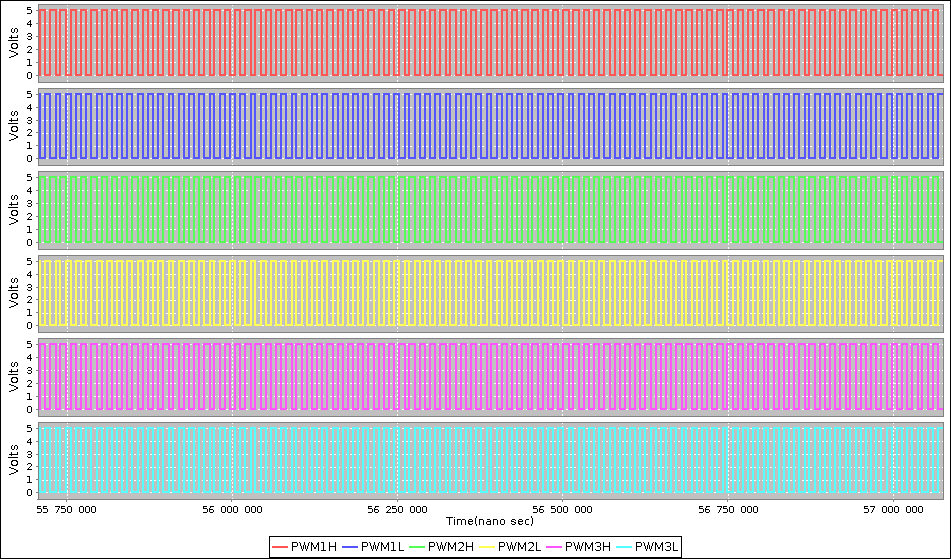
\includegraphics[width=0.9\textwidth]{../Illus/PWM100.png}\hspace*{1em}
	    			\caption{PWM}
	    		 \end{figure}
	  		\end{column}
	  		\begin{column}{0.5\textwidth}
	  			\begin{figure}
	    			\hspace*{1em}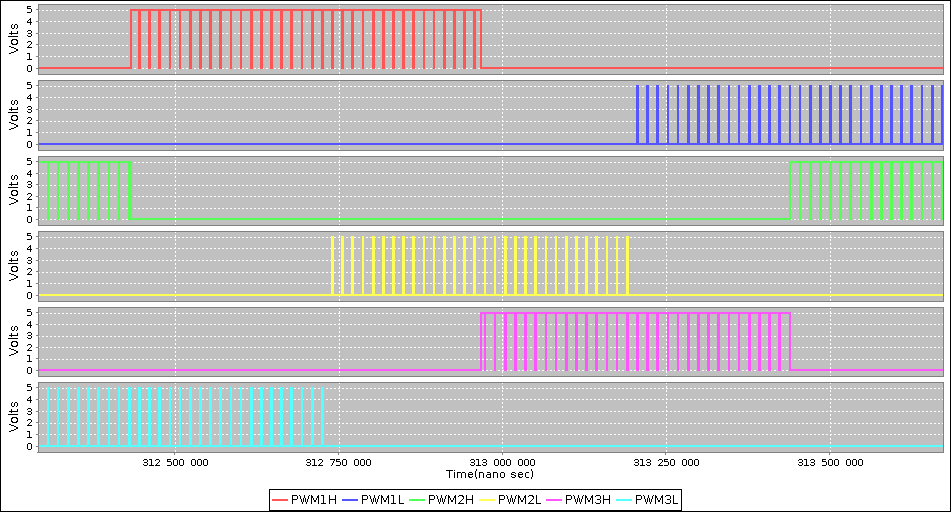
\includegraphics[width=0.9\textwidth]{../Illus/PWMCadence2015.png}\hspace*{1em}
	    			\caption{PWM in Phase Order}
	    		\end{figure}
	  		\end{column}
	  	\end{columns}
	\end{frame}
	
	\author[]{Florian POUTHIER}
	%Intro Power Electronics
	\begin{frame}{Power Electronics}
		\section[ENPU]{Power Electronics}
		Power supply managing and three-phase inverter implementation
 		\begin{itemize}
			\item Functional analysis
			\item \textit{PSIM} simulations
			\item PCB designs
		\end{itemize}
	\end{frame}
	
	% Analyse fonctionnelle
	\begin{frame}{Power Electronics:}
		\framesubtitle{Functional analysis}
		\subsection[Func analysis]{Functional analysis}
		\begin{columns}[T]
	  		\begin{column}{0.4\textwidth}
				\begin{itemize}
					\item \textit{Brushless} motor internal structure
					\item Magnetic laws governing motor's motion settling
					\item Electronic circuit allowing motor control
				\end{itemize}
	  		\end{column}
	  		\begin{column}{0.6\textwidth}
	  			\vspace{-1em}
	  			\begin{figure}
	  				\begin{center}
	  					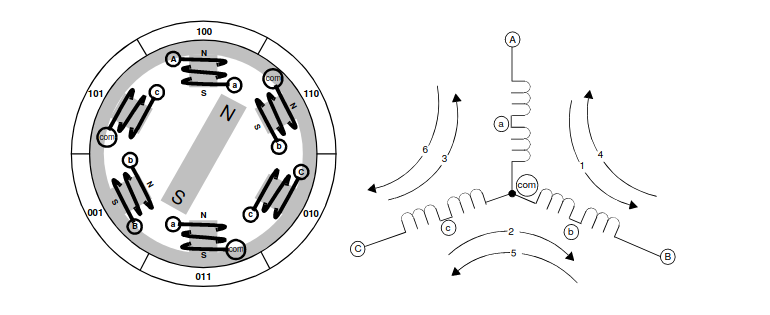
\includegraphics[height=0.3\textheight]{../Illus/struct_bldcm.png}
	  				\end{center}
	    			\caption{\textit{Brushless motor} structure and modelisation}
	    		\end{figure}
	    		\vspace{-2em}
	  			\begin{figure}
	  				\begin{center}
	  					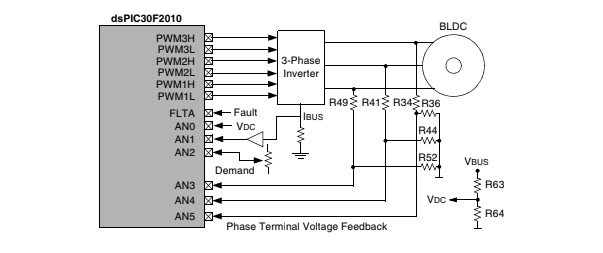
\includegraphics[height=0.3\textheight]{../Illus/back_emf_scheme.png}
	  				\end{center}
	    			\caption{Inverter and back electromagnetic force detection}
	    		\end{figure}
	  		\end{column}
		\end{columns}

	\end{frame}	
		
	% PSIM Simulations - Supply
	\begin{frame}{Power Electronics:}
		\framesubtitle{PSIM simulations}
		\subsection[Simulations]{PSIM simulations}
		\begin{columns}[T]
	  		\begin{column}{0.5\textwidth}
				Simulation of the power supply operation 
				\begin{itemize}
					\item Implementation of the \textit{Buck} based component's internal block diagram
					\item External components definition
					\item Model and external components' values validation
				\end{itemize}
	  		\end{column}
	  		\begin{column}{0.5\textwidth}
	  			\begin{figure}
	  				\begin{center}
	  					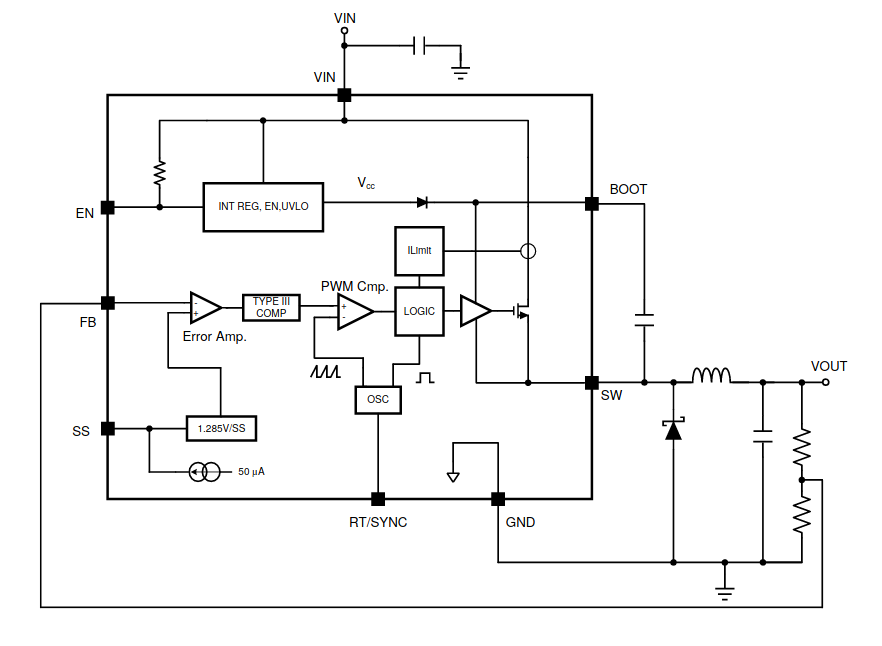
\includegraphics[height=0.5\textheight]{../Illus/func_bloc_lm22672.png}
	  				\end{center}
	    			\caption{LM22672 component's internal block diagram}
	    		\end{figure}
	  		\end{column}
		\end{columns}
	\end{frame}
	
	% PSIM simulations - BLDCM
	\begin{frame}{Power Electronics:}
		\framesubtitle{PSIM simulations}
		\begin{columns}[T]
	  		\begin{column}{0.5\textwidth}
				Simulation of the \textit{brushless} motor operation
				\begin{itemize}
					\item Study of the \textit{brushless} motor steering
					\item Mechanical aspects taken into account with propeller's mathematical modelisation
					\item Hoped propulsion performances verification
				\end{itemize}
	  		\end{column}
	  		\begin{column}{0.5\textwidth}
	  			\begin{figure}
	  				\begin{center}
	  					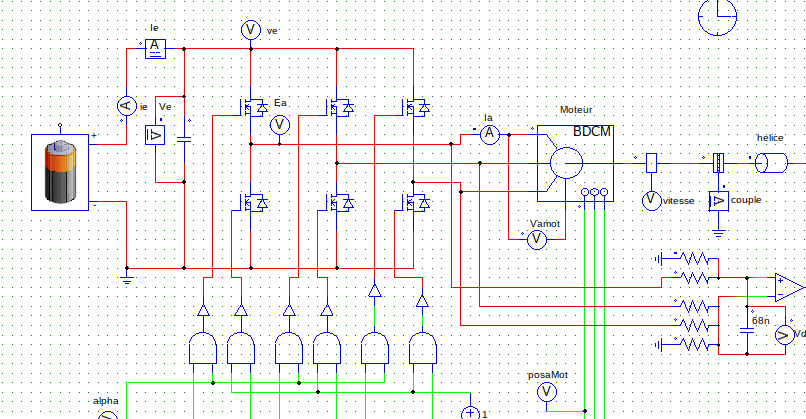
\includegraphics[height=0.35\textheight]{../Illus/simu_bldcm.png}
	  				\end{center}
	    			\caption{\textit{PSIM} implementation of the inverter and \textit{brushless} motor}
	    		\end{figure}
	  		\end{column}
		\end{columns}
	\end{frame}	
	
	% PCB Design - Supply PCB
	\begin{frame}{Power Electronics:}
		\framesubtitle{PCB Design}
		\subsection[PCB Design]{PCB Design}
		\begin{columns}[T]
	  		\begin{column}{0.5\textwidth}
	  			Power supply inteface
		    	\begin{itemize}
		    		\item Obtaining all main voltages required for system operation
		    		\item Electrical ground routed to avoid inrush current
		    		\item Component placement optimization to avoid electromagnetic compatibility
		    	\end{itemize}
	  		\end{column}
	  		\begin{column}{0.5\textwidth}
	  			\begin{figure}
	  				\begin{center}
	  					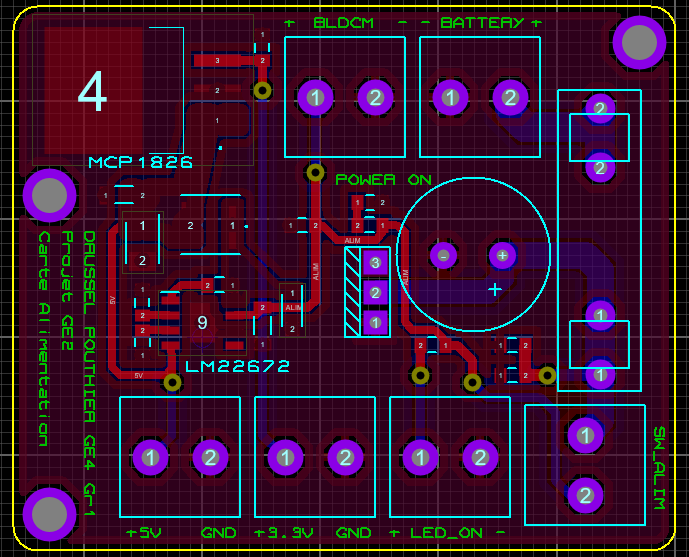
\includegraphics[height=0.5\textheight]{../Illus/PCB_Alim.PNG}
	  				\end{center}
	    			\caption{Power supply PCB view}
	    		\end{figure}
	  		\end{column}
		\end{columns}
	\end{frame}

	% PCB Design - One phase inverter PCB
	\begin{frame}{Power Electronics:}
		\framesubtitle{PCB Design}
		\begin{columns}[T]
	  		\begin{column}{0.6\textwidth}
	  			One phase inverter PCB
		    	\begin{itemize}
		    		\item Heat exchange surfaces determination according to MOSFET losses
		    		\item Use of MOSFET driver to interface PWM control and MOSFET switching
		    		\item Use of decoupling capacitor to avoid inrush currents throw power supply
		    	\end{itemize}
	  		\end{column}
	  		\begin{column}{0.4\textwidth}
	  			\begin{figure}
	  				\begin{center}
	  					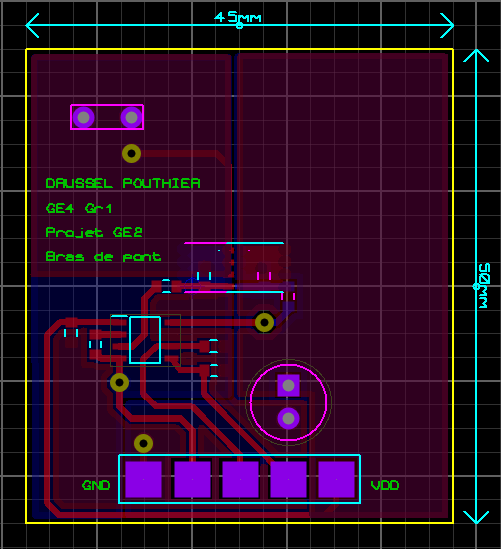
\includegraphics[height=0.5\textheight]{../Illus/PCB_Bras_de_pont.PNG}
	  				\end{center}
	    			\caption{One phase inverter PCB view}
	    		\end{figure}
	  		\end{column}
		\end{columns}
	\end{frame}
	
	% Conception des PCBs - Carte commande
	\begin{frame}{Power Electronics:}
		\framesubtitle{PCB Design}
		\begin{columns}[T]
	  		\begin{column}{0.5\textwidth}
	  			Main control PCB
		    	\begin{itemize}
		    		\item PIC microcontroller operation
		    		\item Managing user input informations received by Bluetooth communication
		    		\item Three phase inverter and servomotor control according to this input informations
		    	\end{itemize}
	  		\end{column}
	  		\begin{column}{0.5\textwidth}
	  			\begin{figure}
	  				\begin{center}
	  					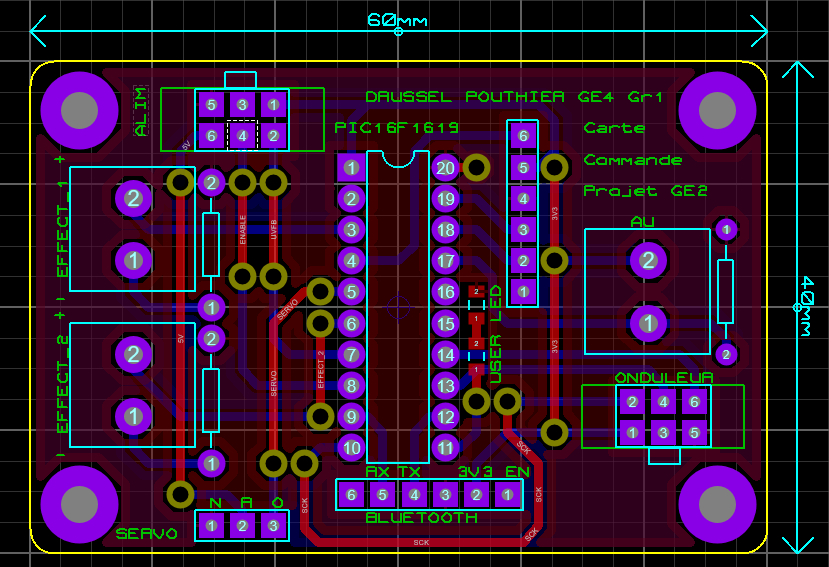
\includegraphics[height=0.4\textheight]{../Illus/PCB_Main.PNG}
	  				\end{center}
	    			\caption{Main control PCB view}
	    		\end{figure}
	  		\end{column}
		\end{columns}
	\end{frame}	
	\begin{frame}{Conclusion}
	\section*{Conclusion}
	%Conclusion
	\begin{itemize}
		    \item Multidisciplinary project
		    \item Use of knowledge and skills previousluy acquired
		\end{itemize}
	\end{frame}
	\author[]{Florian POUTHIER - Tristan DRUSSEL\\ \tiny florian.pouthier@insa-strasbourg.fr - tristan.drussel@insa-strasbourg.fr}

	\begin{frame}[plain]{Thanks!}
	\framesubtitle{Any questions?}
	\section*{}
		%remerciement
		\titlepage
	\end{frame}
\end{document}